\documentclass[10pt]{article}
\usepackage[polish]{babel}
\usepackage[utf8]{inputenc}
\usepackage[T1]{fontenc}
\usepackage{amsmath}
\usepackage{amsfonts}
\usepackage{amssymb}
\usepackage[version=4]{mhchem}
\usepackage{stmaryrd}
\usepackage{graphicx}
\usepackage[export]{adjustbox}
\graphicspath{ {./images/} }
\usepackage{multirow}

\title{Instrukcja dla zdającego }

\author{}
\date{}


\begin{document}
\maketitle
\(\qquad\)\\

\includegraphics[max width=\textwidth, center]{2024_11_21_cce9c7ad32a1dbcd58dag-01}

\[
\text { M А ТЕМАТYKA- klasa } 2 \text { - pp }
\]

\begin{enumerate}
  \item Sprawdź, czy arkusz zawiera 16 stron (zadania 1-34). Ewentualny brak zgłoś przewodniczącemu zespołu nadzorującego egzamin.
  \item Rozwiązania zadań i odpowiedzi zamieść w miejscu na to przeznaczonym.
  \item Odpowiedzi do zadań zamkniętych (1-25) przenieś na kartę odpowiedzi, zaznaczając je w części karty przeznaczonej dla zdającego. Zamaluj pola \(\square\) do tego przeznaczone. Blędne zaznaczenie otocz kółkiem i zaznacz właściwe.
  \item Pamiętaj, że pominięcie argumentacji lub istotnych obliczeń w rozwiązaniu zadania otwartego (26-34) może spowodować, że za to rozwiązanie nie otrzymasz pełnej liczby punktów.
  \item Pisz czytelnie i używaj tylko długopisu lub pióra z czarnym tuszem lub atramentem.
  \item Nie używaj korektora, a błędne zapisy wyraźnie przekreśl.
  \item Pamiętaj, że zapisy w brudnopisie nie będą oceniane.
  \item Możesz korzystać z zestawu wzorów matematycznych, cyrkla i linijki oraz kalkulatora prostego.
  \item Na tej stronie oraz na karcie odpowiedzi wpisz swój kod (nazwisko i imię - zgodnie z ustaleniami szkolnymi).
  \item Nie wpisuj żadnych znaków w części przeznaczonej dla egzaminatora.
\end{enumerate}

Czas pracy:\\
170 minut

Liczba punktów\\
do uzyskania: \(\mathbf{5 0}\)

\section*{Zadanie 1. (1p)}
Wartość wyrażenia \(\left(\frac{3^{-2} \cdot \sqrt[4]{81}}{9^{\frac{1}{2}} \cdot\left(\frac{1}{3}\right)^{3}}\right)^{-1}\) jest równa\\
A. \(3^{-2}\)\\
B. \(3^{-1}\)\\
C. \(3^{1}\)\\
D. \(3^{2}\)

\section*{Zadanie 2. (1p)}
Suma liczby \(x\) i jej kwadratu jest najmniejsza dla liczby \(x\) równej\\
A. -1\\
B. \(\frac{2}{3}\)\\
C. \(\frac{1}{3}\)\\
D. \(-\frac{1}{2}\)

\section*{Zadanie 3. (1p)}
Iloczyn liczby \(\sqrt{3}+1\) i odwrotności liczby \(\sqrt{3}-1\) jest równy\\
A. \(2-\sqrt{3}\)\\
B. \(2+\sqrt{3}\)\\
C. \(2+2 \sqrt{3}\)\\
D. \(2-2 \sqrt{3}\)

\section*{Zadanie 4. (1p)}
Cenę książki obniżano dwukrotnie, najpierw o \(10 \%\), a po miesiącu jeszcze o 5\%. W wyniku obu obniżek cena książki zmniejszyła się o\\
A. \(14 \%\)\\
B. \(15 \%\)\\
C. \(14,5 \%\)\\
D. \(15,5 \%\)

\section*{Zadanie 5. (1p)}
Wartość liczbowa wyrażenia \(5 \log _{2} 2-\log _{2} 8+\log _{2} 16\) jest równa\\
A. 1\\
B. 6\\
C. 2\\
D. 8

\section*{Zadanie 6. (1p)}
Liczba -2 jest miejscem zerowym funkcji \(h(x)=-\frac{1}{2}(2 m-4) x+1\). Wynika stąd, że\\
A. \(m=1,5\)\\
B. \(m=2\)\\
C. \(m=2,5\)\\
D. \(m=1\)

\section*{Zadanie 7. (1p)}
Tangens kąta \(\alpha\) zaznaczonego na rysunku jest równy\\
A. \(\frac{3}{2}\)\\
B. \(-\frac{2}{3}\)\\
C. \(\frac{2}{3}\)\\
D. \(-\frac{3}{2}\)\\
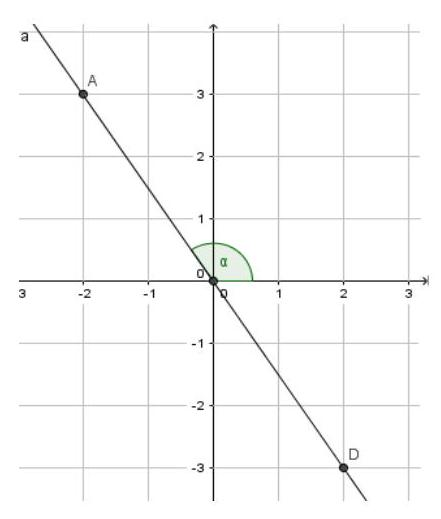
\includegraphics[max width=\textwidth, center]{2024_11_21_cce9c7ad32a1dbcd58dag-02}

\section*{BRUDNOPIS}
\begin{center}
\begin{tabular}{|c|c|c|c|c|c|c|c|c|c|c|c|c|c|c|c|c|c|c|c|}
\hline
 &  &  &  &  &  &  &  &  &  &  &  &  &  &  &  &  &  &  & \multirow[t]{2}{*}{} \\
\hline
 &  &  &  &  &  &  &  &  &  &  &  &  &  &  &  &  &  &  &  \\
\hline
 &  &  &  &  &  &  &  &  &  &  &  &  &  &  &  &  &  &  &  \\
\hline
 &  &  &  &  &  &  &  &  &  &  &  &  &  &  &  &  &  &  &  \\
\hline
 &  &  &  &  &  &  &  &  &  &  &  &  &  &  &  &  &  &  &  \\
\hline
 &  &  &  &  &  &  &  &  &  &  &  &  &  &  &  &  &  &  &  \\
\hline
 &  &  &  &  &  &  &  &  &  &  &  &  &  &  &  &  &  &  &  \\
\hline
 &  &  &  &  &  &  &  &  &  &  &  &  &  &  &  &  &  &  &  \\
\hline
 &  &  &  &  &  &  &  &  &  &  &  &  &  &  &  &  &  &  &  \\
\hline
 &  &  &  &  &  &  &  &  &  &  &  &  &  &  &  &  &  &  &  \\
\hline
 &  &  &  &  &  &  &  &  &  &  &  &  &  &  &  &  &  &  &  \\
\hline
 &  &  &  &  &  &  &  &  &  &  &  &  &  &  &  &  &  &  &  \\
\hline
 &  &  &  &  &  &  &  &  &  &  &  &  &  &  &  &  &  &  &  \\
\hline
 &  &  &  &  &  &  &  &  &  &  &  &  &  &  &  &  &  &  &  \\
\hline
 &  &  &  &  &  &  &  &  &  &  &  &  &  &  &  &  &  &  &  \\
\hline
 &  &  &  &  &  &  &  &  &  &  &  &  &  &  &  &  &  &  &  \\
\hline
 &  &  &  &  &  &  &  &  &  &  &  &  &  &  &  &  &  &  &  \\
\hline
 &  &  &  &  &  &  &  &  &  &  &  &  &  &  &  &  &  &  &  \\
\hline
 &  &  &  &  &  &  &  &  &  &  &  &  &  &  &  &  &  &  &  \\
\hline
 &  &  &  &  &  &  &  &  &  &  &  &  &  &  &  &  &  &  &  \\
\hline
 &  &  &  &  &  &  &  &  &  &  &  &  &  &  &  &  &  &  &  \\
\hline
 &  &  &  &  &  &  &  &  &  &  &  &  &  &  &  &  &  &  &  \\
\hline
 &  &  &  &  &  &  &  &  &  &  &  &  &  &  &  &  &  &  &  \\
\hline
 &  &  &  &  &  &  &  &  &  &  &  &  &  &  &  &  &  &  &  \\
\hline
 &  &  &  &  &  &  &  &  &  &  &  &  &  &  &  &  &  &  &  \\
\hline
 &  &  &  &  &  &  &  &  &  &  &  &  &  &  &  &  &  &  &  \\
\hline
 &  &  &  &  &  &  &  &  &  &  &  &  &  &  &  &  &  &  &  \\
\hline
 &  &  &  &  &  &  &  &  &  &  &  &  &  &  &  &  &  &  &  \\
\hline
 &  &  &  &  &  &  &  &  &  &  &  &  &  &  &  &  &  &  &  \\
\hline
 &  &  &  &  &  &  &  &  &  &  &  &  &  &  &  &  &  &  &  \\
\hline
 &  &  &  &  &  &  &  &  &  &  &  &  &  &  &  &  &  &  &  \\
\hline
 &  &  &  &  &  &  &  &  &  &  &  &  &  &  &  &  &  &  &  \\
\hline
 &  &  &  &  &  &  &  &  &  &  &  &  &  &  &  &  &  &  &  \\
\hline
 &  &  &  &  &  &  &  &  &  &  &  &  &  &  &  &  &  &  &  \\
\hline
 &  &  &  &  &  &  &  &  &  &  &  &  &  &  &  &  &  &  &  \\
\hline
 &  &  &  &  &  &  &  &  &  &  &  &  &  &  &  &  &  &  &  \\
\hline
 &  &  &  &  &  &  &  &  &  &  &  &  &  &  &  &  &  &  &  \\
\hline
 &  &  &  &  &  &  &  &  &  &  &  &  &  &  &  &  &  &  &  \\
\hline
 &  &  &  &  &  &  &  &  &  &  &  &  &  &  &  &  &  &  &  \\
\hline
 &  &  &  &  &  &  &  &  &  &  &  &  &  &  &  &  &  &  &  \\
\hline
 &  &  &  &  &  &  &  &  &  &  &  &  &  &  &  &  &  &  &  \\
\hline
 &  &  &  &  &  &  &  &  &  &  &  &  &  &  &  &  &  &  &  \\
\hline
 &  &  &  &  &  &  &  &  &  &  &  &  &  &  &  &  &  &  &  \\
\hline
\end{tabular}
\end{center}

Zadanie 8. (1p)\\
Zbiorem wartości funkcji, której wykres przedstawiono na rysunku jest\\
A. \((-2,2)\)\\
B. \((-2,2)\)\\
C. \((-2,2)\)\\
D. \(\langle-2,2\rangle\)\\
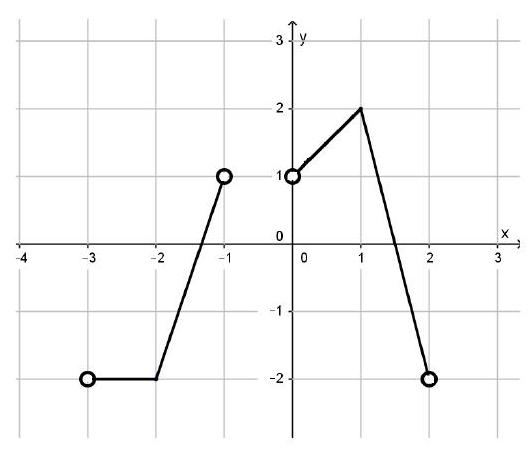
\includegraphics[max width=\textwidth, center]{2024_11_21_cce9c7ad32a1dbcd58dag-04(1)}

\section*{Zadanie 9. (1p)}
Obwód trójkąta równobocznego jest równy \(\frac{6 x}{y}\), gdzie \(x>0, y>0\). Pole powierzchni tego trójkąta jest równe\\
A. \(\frac{3 x}{y}\)\\
B. \(\frac{x^{2} \sqrt{3}}{y^{2}}\)\\
C. \(\frac{x^{2}}{y^{2}}\)\\
D. \(\frac{x \sqrt{3}}{y}\)

Zadanie 10. (1p)\\
Dziedziną funkcji \(f(x)=\frac{x-2}{\sqrt{x-2}}+\frac{2-x}{x}\) jest\\
A. \(x \neq 2\)\\
B. \(x \neq 0\)\\
C. \(x>2\)\\
D. \(x \in R\)

\section*{Zadanie 11. (1p)}
Miara kąta \(\alpha\) pod jakim przecinają się styczne do okręgu o środku S wynosi\\
A. \(60^{\circ}\)\\
B. \(30^{\circ}\)\\
C. \(40^{\circ}\)\\
D. \(45^{\circ}\)\\
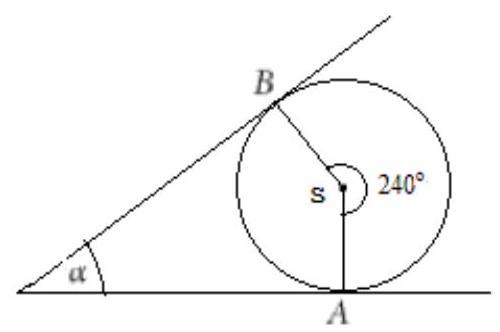
\includegraphics[max width=\textwidth, center]{2024_11_21_cce9c7ad32a1dbcd58dag-04}

Zadanie 12. (1p)\\
Jeżeli \(f(x)=x+1\) i \(g(x)=f(x-1)+2\), to funkcja \(g(x)\) jest równa\\
A. \(-x+2\)\\
B. \(-x-2\)\\
C. \(x-2\)\\
D. \(x+2\)

\section*{Zadanie 13. (1p)}
Wśród podanych poniżej nierówności wskaż tę, której zbiorem rozwiązań jest przedział \((-6,8)\)\\
A. \(8<x-2<-6\)\\
B. \(-6<x-2<8\)\\
C. \(-8<x-2<6\)\\
D. \(-8<x+2<6\)

\section*{BRUDNOPIS}
Zadanie 14. (1p)\\
Punkt \(A=(2 ; 7)\) jest wierzchołkiem kwadratu \(A B C D\), a punkt \(S=(6 ; 5)\) jest środkiem okręgu opisanego na tym kwadracie. Bok tego kwadratu ma długość\\
A. \(\sqrt{20}\)\\
B. \(2 \sqrt{20}\)\\
C. \(\sqrt{10}\)\\
D. \(2 \sqrt{10}\)

\section*{Zadanie 15. (1p)}
Wiadomo, że \(\sin \alpha=\frac{3 \sqrt{5}}{7}\) i \(\alpha \in\left(90^{\circ} ; 180^{\circ}\right)\). Wynika stąd, że\\
A. \(\cos \alpha=-\frac{4}{49}\)\\
B. \(\cos \alpha=\frac{2}{7}\)\\
C. \(\cos \alpha=-\frac{2}{7}\)\\
D. \(\cos \alpha=-\frac{\sqrt{34}}{7}\)

\section*{Zadanie 16. (1p)}
Kąty ABC i ADE są równe oraz \(|A B|=x-3,|B D|=x\), \(|B C|=2,|D E|=8\). Wobec tego x jest równe\\
A. 3\\
B. 3,5\\
C. 4,5\\
D. 4\\
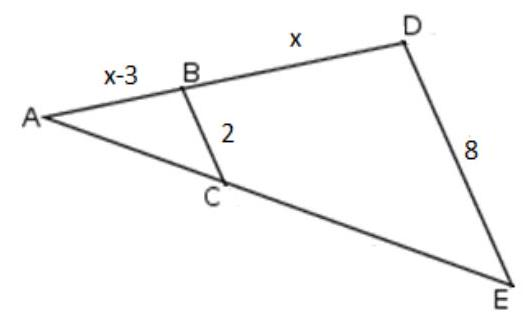
\includegraphics[max width=\textwidth, center]{2024_11_21_cce9c7ad32a1dbcd58dag-06}

\section*{Zadanie 17. (1p)}
Dany jest trzywyrazowy ciąg geometryczny o wyrazach dodatnich: \((2, x \sqrt{2}, 6)\). Wówczas\\
A. \(x=\sqrt{6}\)\\
B. \(x=6\)\\
C. \(x=3\)\\
D. \(x=3 \sqrt{2}\)

Zadanie 18. (1p)\\
Dany jest ciąg liczbowy \(\left(a_{n}\right)\), w którym, \(a_{1}=x-1, a_{2}=2 x+1, a_{3}=4 x+1\).\\
Dla jakiej wartości liczbowej \(x\) dany ciąg jest ciągiem arytmetycznym?\\
A. \(x=-2\)\\
B. 2\\
C. 3\\
D. 4

Zadanie 19. (1p)\\
Jeżeli \(x \in\langle-2 ; 0)\), to wartość wyrażenia \(3 x-|x+2|+|x|\) jest równa\\
A. \(x+2\)\\
B. \(3 x+2\)\\
C. \(x-2\)\\
D. \(5 x+2\)

Zadanie 20. (1p)\\
Setny wyraz ciągu \(\left(\boldsymbol{a}_{\boldsymbol{n}}\right)\) jest równy 2018. Wzór ogólny na n-ty wyraz ciągu ( \(\boldsymbol{a}_{\boldsymbol{n}}\) ) może mieć postać\\
A. \(a_{n}=2 n-2018\)\\
B. \(a_{n}=n^{2}-100 n\)\\
C. \(a_{n}=\frac{n^{2}}{4}-482\)\\
D. \(a_{n}=\frac{n+2018}{n}\)

\section*{Zadanie 21. (1p)}
Do wykresu funkcji \(f\) danej wzorem \(f(x)=3^{x}-4\) należy punkt o współrzędnych\\
A. \((-1,-7)\)\\
B. \((0,-3)\)\\
C. \((0,-4)\)\\
D. \((2,2)\)

\section*{Zadanie 22. (1p)}
Piąty wyraz rosnącego ciągu geometrycznego jest równy \(5 \frac{1}{3}\), a siódmy \(21 \frac{1}{3}\). Iloraz tego ciągu jest równy\\
A. -4\\
B. -2\\
C. 4\\
D. 2

Zadanie 23. (1p)\\
Na okręgu o środku w punkcie \(O\) leżą punkty \(A, B, C\) (zobacz rysunek). Odcinek \(A C\) jest średnicą okręgu. Kąt \(A O B\) ma miarę \(58^{\circ}\). Kąt \(O B C\) ma miarę równą\\
A. \(39^{\circ}\)\\
B. \(31^{\circ}\)\\
C. \(29^{\circ}\)\\
D. \(41^{\circ}\)\\
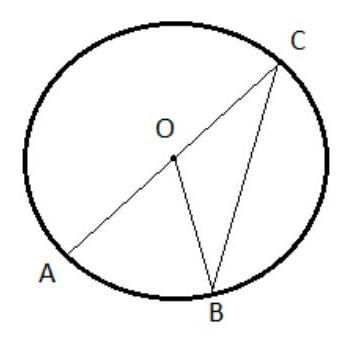
\includegraphics[max width=\textwidth, center]{2024_11_21_cce9c7ad32a1dbcd58dag-07(1)}

\section*{Zadanie 24. (1p)}
W trapezie równoramiennym (patrz rysunek obok) tangens kąta ostrego \(\alpha\) jest równy\\
A. \(\frac{\sqrt{3}}{3}\)\\
B. \(\frac{\sqrt{2}}{2}\)\\
C. \(\sqrt{3}\)\\
D. \(\sqrt{2}\)\\
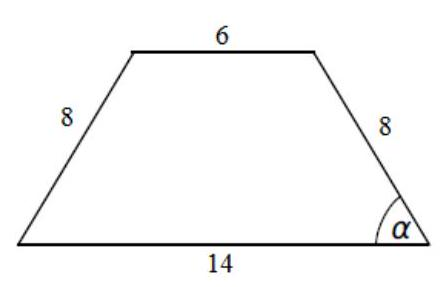
\includegraphics[max width=\textwidth, center]{2024_11_21_cce9c7ad32a1dbcd58dag-07}

\section*{Zadanie 25. (1p)}
Funkcja kwadratowa określona jest wzorem \(f(x)=-x^{2}+2 x+c\). Jeżeli \(f(4)=-2\), to\\
A. \(f(1)=5\)\\
B. \(f(1)=7\)\\
C. \(f(1)=-7\)\\
D. \(f(1)=-5\)

\section*{BRUDNOPIS}
\begin{center}

\includegraphics[max width=\textwidth]{2024_11_21_cce9c7ad32a1dbcd58dag-07(2)}
\end{center}

\section*{BRUDNOPIS}
\begin{center}

\includegraphics[max width=\textwidth]{2024_11_21_cce9c7ad32a1dbcd58dag-08}
\end{center}

\section*{LUBELSKA PRÓBA PRZED MATURĄ - klasa 2 - poziom podstawowy}
\section*{ZADANIA OTWARTE}
Rozwiązania zadań o numerach od 26 do 34 należy zapisać \(w\) wyznaczonych miejscach pod treścia zadania (pamiętaj o udzieleniu odpowiedzi)

\section*{Zadanie 26. (2p)}
Wyznacz zbiór niedodatnich rozwiązań nierówności \(-x^{2}+15 \geq 2 x\).\\

\includegraphics[max width=\textwidth, center]{2024_11_21_cce9c7ad32a1dbcd58dag-09(2)}

Odpowiedź:

\section*{Zadanie 27. (2p)}
Wykaż, że trójkąt o wierzchołkach \(A=(1,2), B=(6,3), C=(4,5)\) jest prostokątny.\\

\includegraphics[max width=\textwidth, center]{2024_11_21_cce9c7ad32a1dbcd58dag-09}

Odpowiedź:\\
Zadanie 28. (2p)\\
Oblicz obwód trójkąta prostokątnego o polu powierzchni równym \(35 \mathrm{~cm}^{2}\), wiedząc, że długości jego przyprostokątnych różnią się o 3 cm .\\

\includegraphics[max width=\textwidth, center]{2024_11_21_cce9c7ad32a1dbcd58dag-09(1)}

Odpowiedź:

\section*{Zadanie 29. (2p)}
Wyrazami ciągu arytmetycznego \(\left(a_{n}\right)\) są kolejne liczby naturalne, które przy dzieleniu przez 5 dają resztę 3. Ponadto \(a_{6}=28\). Oblicz \(a_{15}\)\\

\includegraphics[max width=\textwidth, center]{2024_11_21_cce9c7ad32a1dbcd58dag-10}

\section*{Zadanie 30. (2p)}
Ojciec i syn mają łącznie 50 lat. 5 lat temu ojciec był trzykrotnie starszy od syna. Ile lat ma ojciec, a ile syn?\\

\includegraphics[max width=\textwidth, center]{2024_11_21_cce9c7ad32a1dbcd58dag-10(1)}

Zadanie 31. (2p)\\
Wykaż, że jeżeli środkowa trójkąta jest dwa razy krótsza od boku, do którego jest poprowadzona, to trójkąt ten jest prostokątny.

Zadanie 32. (4p)\\
Na prostej o równaniu \(y=x\) wyznacz współrzędne punktu P leżącego najbliżej punktu \(K=(-1 ; 7)\).\\

\includegraphics[max width=\textwidth, center]{2024_11_21_cce9c7ad32a1dbcd58dag-11}

Odpowiedź:

\section*{Zadanie 33. (4p)}
W wyniku zwiększenia każdego boku danego prostokąta o 2 cm jego pole wzrosło o \(20 \mathrm{~cm}^{2}\). O ile \(\mathrm{cm}^{2}\) zwiększy się pole danego prostokąta, jeśli jego boki zwiększymy o 3 cm ?\\

\includegraphics[max width=\textwidth, center]{2024_11_21_cce9c7ad32a1dbcd58dag-11(1)}

Odpowiedź:

Zadanie 34. (5p)\\
Na okręgu o promieniu 3 opisano trójkąt prostokątny o jednej z przyprostokątnych długości 12. Oblicz obwód tego trójkąta.

Odpowiedź:

\section*{BRUDNOPIS}
\begin{center}
\begin{tabular}{|c|c|c|c|c|c|c|c|c|c|c|c|c|c|c|c|c|c|c|c|c|}
\hline
 &  &  &  &  &  &  &  &  &  &  &  &  &  &  &  &  &  &  &  &  \\
\hline
 &  &  &  &  &  &  &  &  &  &  &  &  &  &  &  &  &  &  &  &  \\
\hline
 &  &  &  &  &  &  &  &  &  &  &  &  &  &  &  &  &  &  &  &  \\
\hline
 &  &  &  &  &  &  &  &  &  &  &  &  &  &  &  &  &  &  &  &  \\
\hline
 &  &  &  &  &  &  &  &  &  &  &  &  &  &  &  &  &  &  &  &  \\
\hline
 &  &  &  &  &  &  &  &  &  &  &  &  &  &  &  &  &  &  &  &  \\
\hline
 &  &  &  &  &  &  &  &  &  &  &  &  &  &  &  &  &  &  &  &  \\
\hline
 &  &  &  &  &  &  &  &  &  &  &  &  &  &  &  &  &  &  &  &  \\
\hline
 &  &  &  &  &  &  &  &  &  &  &  &  &  &  &  &  &  &  &  &  \\
\hline
 &  &  &  &  &  &  &  &  &  &  &  &  &  &  &  &  &  &  &  &  \\
\hline
 &  &  &  &  &  &  &  &  &  &  &  &  &  &  &  &  &  &  &  &  \\
\hline
 &  &  &  &  &  &  &  &  &  &  &  &  &  &  &  &  &  &  &  &  \\
\hline
 &  &  &  &  &  &  &  &  &  &  &  &  &  &  &  &  &  &  &  &  \\
\hline
 &  &  &  &  &  &  &  &  &  &  &  &  &  &  &  &  &  &  &  &  \\
\hline
 &  &  &  &  &  &  &  &  &  &  &  &  &  &  &  &  &  &  &  &  \\
\hline
 &  &  &  &  &  &  &  &  &  &  &  &  &  &  &  &  &  &  &  &  \\
\hline
 &  &  &  &  &  &  &  &  &  &  &  &  &  &  &  &  &  &  &  &  \\
\hline
 &  &  &  &  &  &  &  &  &  &  &  &  &  &  &  &  &  &  &  &  \\
\hline
 &  &  &  &  &  &  &  &  &  &  &  &  &  &  &  &  &  &  &  &  \\
\hline
 &  &  &  &  &  &  &  &  &  &  &  &  &  &  &  &  &  &  &  &  \\
\hline
 &  &  &  &  &  &  &  &  &  &  &  &  &  &  &  &  &  &  &  &  \\
\hline
 &  &  &  &  &  &  &  &  &  &  &  &  &  &  &  &  &  &  &  &  \\
\hline
 &  &  &  &  &  &  &  &  &  &  &  &  &  &  &  &  &  &  &  &  \\
\hline
 &  &  &  &  &  &  &  &  &  &  &  &  &  &  &  &  &  &  &  &  \\
\hline
 &  &  &  &  &  &  &  &  &  &  &  &  &  &  &  &  &  &  &  &  \\
\hline
 &  &  &  &  &  &  &  &  &  &  &  &  &  &  &  &  &  &  &  &  \\
\hline
 &  &  &  &  &  &  &  &  &  &  &  &  &  &  &  &  &  &  &  &  \\
\hline
 &  &  &  &  &  &  &  &  &  &  &  &  &  &  &  &  &  &  &  &  \\
\hline
 &  &  &  &  &  &  &  &  &  &  &  &  &  &  &  &  &  &  &  &  \\
\hline
 &  &  &  &  &  &  &  &  &  &  &  &  &  &  &  &  &  &  &  &  \\
\hline
 &  &  &  &  &  &  &  &  &  &  &  &  &  &  &  &  &  &  &  &  \\
\hline
 &  &  &  &  &  &  &  &  &  &  &  &  &  &  &  &  &  &  &  &  \\
\hline
 &  &  &  &  &  &  &  &  &  &  &  &  &  &  &  &  &  &  &  &  \\
\hline
 &  &  &  &  &  &  &  &  &  &  &  &  &  &  &  &  &  &  &  &  \\
\hline
 &  &  &  &  &  &  &  &  &  &  &  &  &  &  &  &  &  &  &  &  \\
\hline
 &  &  &  &  &  &  &  &  &  &  &  &  &  &  &  &  &  &  &  &  \\
\hline
 &  &  &  &  &  &  &  &  &  &  &  &  &  &  &  &  &  &  &  &  \\
\hline
 &  &  &  &  &  &  &  &  &  &  &  &  &  &  &  &  &  &  &  &  \\
\hline
 &  &  &  &  &  &  &  &  &  &  &  &  &  &  &  &  &  &  &  &  \\
\hline
 &  &  &  &  &  &  &  &  &  &  &  &  &  &  &  &  &  &  &  &  \\
\hline
 &  &  &  &  &  &  &  &  &  &  &  &  &  &  &  &  &  &  &  &  \\
\hline
 &  &  &  &  &  &  &  &  &  &  &  &  &  &  &  &  &  &  &  &  \\
\hline
 &  &  &  &  &  &  &  &  &  &  &  &  &  &  &  &  &  &  &  &  \\
\hline
\end{tabular}
\end{center}

\section*{BRUDNOPIS}
\begin{center}

\includegraphics[max width=\textwidth]{2024_11_21_cce9c7ad32a1dbcd58dag-14}
\end{center}

\section*{BRUDNOPIS}
\begin{center}
\begin{tabular}{|c|c|c|c|c|c|c|c|c|c|c|c|c|c|c|c|c|c|c|c|c|}
\hline
 &  &  &  &  &  &  &  &  &  &  &  &  &  &  &  &  &  &  &  &  \\
\hline
 &  &  &  &  &  &  &  &  &  &  &  &  &  &  &  &  &  &  &  &  \\
\hline
 &  &  &  &  &  &  &  &  &  &  &  &  &  &  &  &  &  &  &  &  \\
\hline
 &  &  &  &  &  &  &  &  &  &  &  &  &  &  &  &  &  &  &  &  \\
\hline
 &  &  &  &  &  &  &  &  &  &  &  &  &  &  &  &  &  &  &  &  \\
\hline
 &  &  &  &  &  &  &  &  &  &  &  &  &  &  &  &  &  &  &  &  \\
\hline
 &  &  &  &  &  &  &  &  &  &  &  &  &  &  &  &  &  &  &  &  \\
\hline
 &  &  &  &  &  &  &  &  &  &  &  &  &  &  &  &  &  &  &  &  \\
\hline
 &  &  &  &  &  &  &  &  &  &  &  &  &  &  &  &  &  &  &  &  \\
\hline
 &  &  &  &  &  &  &  &  &  &  &  &  &  &  &  &  &  &  &  &  \\
\hline
 &  &  &  &  &  &  &  &  &  &  &  &  &  &  &  &  &  &  &  &  \\
\hline
 &  &  &  &  &  &  &  &  &  &  &  &  &  &  &  &  &  &  &  &  \\
\hline
 &  &  &  &  &  &  &  &  &  &  &  &  &  &  &  &  &  &  &  &  \\
\hline
 &  &  &  &  &  &  &  &  &  &  &  &  &  &  &  &  &  &  &  &  \\
\hline
 &  &  &  &  &  &  &  &  &  &  &  &  &  &  &  &  &  &  &  &  \\
\hline
 &  &  &  &  &  &  &  &  &  &  &  &  &  &  &  &  &  &  &  &  \\
\hline
 &  &  &  &  &  &  &  &  &  &  &  &  &  &  &  &  &  &  &  &  \\
\hline
 &  &  &  &  &  &  &  &  &  &  &  &  &  &  &  &  &  &  &  &  \\
\hline
 &  &  &  &  &  &  &  &  &  &  &  &  &  &  &  &  &  &  &  &  \\
\hline
 &  &  &  &  &  &  &  &  &  &  &  &  &  &  &  &  &  &  &  &  \\
\hline
 &  &  &  &  &  &  &  &  &  &  &  &  &  &  &  &  &  &  &  &  \\
\hline
 &  &  &  &  &  &  &  &  &  &  &  &  &  &  &  &  &  &  &  &  \\
\hline
 &  &  &  &  &  &  &  &  &  &  &  &  &  &  &  &  &  &  &  &  \\
\hline
 &  &  &  &  &  &  &  &  &  &  &  &  &  &  &  &  &  &  &  &  \\
\hline
 &  &  &  &  &  &  &  &  &  &  &  &  &  &  &  &  &  &  &  &  \\
\hline
 &  &  &  &  &  &  &  &  &  &  &  &  &  &  &  &  &  &  &  &  \\
\hline
 &  &  &  &  &  &  &  &  &  &  &  &  &  &  &  &  &  &  &  &  \\
\hline
 &  &  &  &  &  &  &  &  &  &  &  &  &  &  &  &  &  &  &  &  \\
\hline
 &  &  &  &  &  &  &  &  &  &  &  &  &  &  &  &  &  &  &  &  \\
\hline
 &  &  &  &  &  &  &  &  &  &  &  &  &  &  &  &  &  &  &  &  \\
\hline
 &  &  &  &  &  &  &  &  &  &  &  &  &  &  &  &  &  &  &  &  \\
\hline
 &  &  &  &  &  &  &  &  &  &  &  &  &  &  &  &  &  &  &  &  \\
\hline
 &  &  &  &  &  &  &  &  &  &  &  &  &  &  &  &  &  &  &  &  \\
\hline
 &  &  &  &  &  &  &  &  &  &  &  &  &  &  &  &  &  &  &  &  \\
\hline
 &  &  &  &  &  &  &  &  &  &  &  &  &  &  &  &  &  &  &  &  \\
\hline
 &  &  &  &  &  &  &  &  &  &  &  &  &  &  &  &  &  &  &  &  \\
\hline
 &  &  &  &  &  &  &  &  &  &  &  &  &  &  &  &  &  &  &  &  \\
\hline
 &  &  &  &  &  &  &  &  &  &  &  &  &  &  &  &  &  &  &  &  \\
\hline
 &  &  &  &  &  &  &  &  &  &  &  &  &  &  &  &  &  &  &  &  \\
\hline
 &  &  &  &  &  &  &  &  &  &  &  &  &  &  &  &  &  &  &  &  \\
\hline
 &  &  &  &  &  &  &  &  &  &  &  &  &  &  &  &  &  &  &  &  \\
\hline
 &  &  &  &  &  &  &  &  &  &  &  &  &  &  &  &  &  &  &  &  \\
\hline
 &  &  &  &  &  &  &  &  &  &  &  &  &  &  &  &  &  &  &  &  \\
\hline
\end{tabular}
\end{center}

\section*{KARTA ODPOWIEDZI}
KOD UCZNIA\\
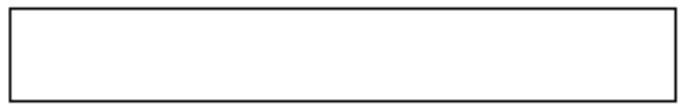
\includegraphics[max width=\textwidth, center]{2024_11_21_cce9c7ad32a1dbcd58dag-16}

Wypełnia piszący\\
Wypelnia sprawdzający

\begin{center}
\begin{tabular}{|c|c|c|c|c|}
\hline
\begin{tabular}{c}
Nr \\
zadmia \\
\end{tabular} & A & B & C & D \\
\hline
1. & \(\square\) & \(\square\) & \(\square\) & \(\square\) \\
\hline
2. & \(\square\) & \(\square\) & \(\square\) & \(\square\) \\
\hline
3. & \(\square\) & \(\square\) & \(\square\) & \(\square\) \\
\hline
4. & \(\square\) & \(\square\) & \(\square\) & \(\square\) \\
\hline
5. & \(\square\) & \(\square\) & \(\square\) & \(\square\) \\
\hline
6. & \(\square\) & \(\square\) & \(\square\) & \(\square\) \\
\hline
7. & \(\square\) & \(\square\) & \(\square\) & \(\square\) \\
\hline
8. & \(\square\) & \(\square\) & \(\square\) & \(\square\) \\
\hline
9. & \(\square\) & \(\square\) & \(\square\) & \(\square\) \\
\hline
10. & \(\square\) & \(\square\) & \(\square\) & \(\square\) \\
\hline
11. & \(\square\) & \(\square\) & \(\square\) & \(\square\) \\
\hline
12. & \(\square\) & \(\square\) & \(\square\) & \(\square\) \\
\hline
13. & \(\square\) & \(\square\) & \(\square\) & \(\square\) \\
\hline
14. & \(\square\) & \(\square\) & \(\square\) & \(\square\) \\
\hline
15. & \(\square\) & \(\square\) & \(\square\) & \(\square\) \\
\hline
16. & \(\square\) & \(\square\) & \(\square\) & \(\square\) \\
\hline
17. & \(\square\) & \(\square\) & \(\square\) & \(\square\) \\
\hline
18. & \(\square\) & \(\square\) & \(\square\) & \(\square\) \\
\hline
19. & \(\square\) & \(\square\) & \(\square\) & \(\square\) \\
\hline
20. & \(\square\) & \(\square\) & \(\square\) & \(\square\) \\
\hline
21. & \(\square\) & \(\square\) & \(\square\) & \(\square\) \\
\hline
22. & \(\square\) & \(\square\) & \(\square\) & \(\square\) \\
\hline
23. & \(\square\) & \(\square\) & \(\square\) & \(\square\) \\
\hline
24. & \(\square\) & \(\square\) & \(\square\) & \(\square\) \\
\hline
25. & \(\square\) & \(\square\) & \(\square\) & \(\square\) \\
\hline
\end{tabular}
\end{center}

\begin{center}
\begin{tabular}{|c|c|c|c|c|}
\hline
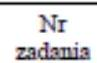
\includegraphics[max width=\textwidth]{2024_11_21_cce9c7ad32a1dbcd58dag-16(1)}
 & X & 0 & 1 & 2 \\
\hline
26. & ㅁ & ㅁ & ㅁ & ㅁ \\
\hline
27. & ㅁ & ㅁ & ■ & ㅁ \\
\hline
28. & ㅁ & ㅁ & ㅁ & ㅁ \\
\hline
29. & ㅁ & ㅁ & ■ & ㅁ \\
\hline
30. & ㅁ & ㅁ & ㅁ & ■ \\
\hline
31. & ㅁ & - & ㅁ & ㅁ \\
\hline
\multicolumn{5}{|c|}{Razem} \\
\hline
\end{tabular}
\end{center}

\begin{center}
\begin{tabular}{|c|c|c|c|c|c|c|c|}
\hline
\begin{tabular}{c}
Nr \\
zdamia \\
\end{tabular} & X & 0 & 1 & 2 & 3 & 4 & 5 \\
\hline
32. & \(\square\) & \(\square\) & \(\square\) & \(\square\) & \(\square\) & \(\square\) &  \\
\hline
33. & \(\square\) & \(\square\) & \(\square\) & \(\square\) & \(\square\) & \(\square\) &  \\
\hline
34. & \(\square\) & \(\square\) & \(\square\) & \(\square\) & \(\square\) & \(\square\) & \(\square\) \\
\hline
\end{tabular}
\end{center}

Razem

\begin{center}
\begin{tabular}{|l|l|}
\hline
Suma punktów & Wynik w \% \\
\hline
 &  \\
 &  \\
\hline
\end{tabular}
\end{center}

Razem\\
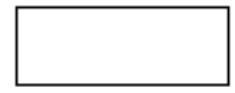
\includegraphics[max width=\textwidth, center]{2024_11_21_cce9c7ad32a1dbcd58dag-16(2)}


\end{document}